\documentclass[aps,amssymb,amsmath,prl,superscriptaddress,reprint,noshowpacs]{revtex4-1}


\usepackage{times}
\usepackage{amssymb,amsmath,graphicx}
\usepackage[usenames]{color}
%\usepackage{pdfpages}
\usepackage{bbold}
\usepackage{siunitx}
\usepackage{braket}
\usepackage{comment}
\usepackage[T1]{fontenc}
\usepackage[utf8]{inputenc}
\usepackage[english]{babel}
\usepackage{etoolbox}
\usepackage{lipsum} 

\usepackage{hyperref}
\hypersetup{colorlinks=true, citecolor=blue, urlcolor=blue, linkcolor=blue}

%%%%%%%%%%%%%%%%%%%%% New for revision
\usepackage[normalem]{ulem}
\usepackage{lineno}
%\linenumbers
%%%%%%%%%%%%%%%%%%%%%


%%%%% This is just for the extended data table 1
%%%%% remove for a new document!!!
%\usepackage[tablename=Extended~Data~Table]{caption}
%%%%%%



\newcommand{\Og}{\ensuremath{\Omega}}
\newcommand{\Oo}{\Omega_\mathrm{0}}
\newcommand{\Om}{\Omega_\mathrm{m}}
\newcommand{\Oe}{\Omega_\mathrm{e}}
\newcommand{\Ox}{\Omega_\mathrm{x}}
\newcommand{\Oy}{\Omega_\mathrm{y}}
\newcommand{\Oz}{\Omega_\mathrm{z}}
\newcommand{\Gm}{\gamma_\mathrm{m}}
\newcommand{\Gth}{\Gamma_\mathrm{th}}
\newcommand{\Gtot}{\Gamma_\mathrm{tot}}
\newcommand{\Gexc}{\Gamma_\mathrm{exc}}
\newcommand{\Geff}{\gamma_\mathrm{eff}}
\newcommand{\Gfb}{\gamma_\mathrm{fb}}
\newcommand{\Gmeas}{\Gamma_\mathrm{meas}}
\newcommand{\Gqba}{\Gamma_\mathrm{qba}}
\newcommand{\etadet}{\eta_d}
\newcommand{\etameas}{\eta_\mathrm{meas}}
\newcommand{\nbar}{\overline{n}}
\newcommand{\Sbar}{\overline{S}}
\newcommand{\Sfftot}{\Sbar_{FF}^\text{tot}}
\newcommand{\Simp}{\Sbar_\text{imp}}
\newcommand{\zzpf}{z_\mathrm{zpf}}
\newcommand{\pzpf}{p_\mathrm{zpf}}
\newcommand{\NA}{\mathrm{N \mskip-0.5\thinmuskip A}}
\newcommand{\vect}[1]{\boldsymbol{#1}}
\newcommand{\abs}[1]{\left| #1 \right|} % for absolute value
%\newcommand{\vect}[1]{\mathbf{#1}}
\newcommand{\RE}[1]{\operatorname{Re}\{#1\}}
\newcommand{\IM}[1]{\operatorname{Im}\{#1\}}
\newcommand{\imu}{\text{\rm i}}
\newcommand{\expu}{\text{\rm e}}
\newcommand{\diff}{\text{d}}

% textcomp, for its upright mu
\usepackage{textcomp}
% some user macros
\newcommand{\murm}{\hbox{\textmu}}

\newcommand{\figwidth}{0.95\columnwidth} %% specifies size for pictures
\newcommand{\commentOut}[1]{}
\usepackage{scalefnt}   % to scale font size

\newcommand{\affil}{Photonics Laboratory, ETH Zürich, CH-8093 Zürich, Switzerland}
\newcommand{\affilQC}{Quantum Center, ETH Zürich, CH-8093 Zürich, Switzerland}
\newcommand{\affilICFO}{
ICFO -- Institut de Ciencies Fotoniques, The Barcelona Institute of Science and Technology, Castelldefels,
Barcelona 08860, Spain}
\newcommand{\affilICREA}{
ICREA -- Institucio Catalana de Recerca i Estudis Avancats, Barcelona 08010, Spain}
\newcommand{\affilIQOQI}{
Institute for Quantum Optics and Quantum Information of the Austrian Academy of Sciences, A-6020 Innsbruck, Austria}
\newcommand{\affilITP}{
2Institute for Theoretical Physics, University of Innsbruck, A-6020 Innsbruck, Austria}



\begin{document}
\scalefont{1.05}
\title{Quantum Delocalization of a Levitated Nanoparticle}

\author{M. Rossi}
\altaffiliation{Present address: Kavli Institute of Nanoscience, Department of Quantum Nanoscience, Delft University of Technology, 2628CJ Delft, The Netherlands}
\affiliation{\affil}
\affiliation{\affilQC}

\author{A. Militaru}
\altaffiliation{Present address: Institute of Science and Technology Austria, Am Campus 1, 3400 Klosterneuburg, Austria}
\affiliation{\affil}
\affiliation{\affilQC}

\author{N. Carlon Zambon}
\affiliation{\affil}
\affiliation{\affilQC}

\author{\\A.~Riera-Campeny}
\affiliation{\affilICFO}
\affiliation{\affilIQOQI}

\author{O. Romero-Isart}
\affiliation{\affilICFO}
\affiliation{\affilICREA}

\author{M. Frimmer}
\affiliation{\affil}
\affiliation{\affilQC}

\author{L. Novotny}
\affiliation{\affil}
\affiliation{\affilQC}

% \date\today
\begin{abstract}
Every massive particle behaves like a wave, according to quantum physics. Yet, this characteristic wave nature has only been observed in double-slit experiments with microscopic systems, such as atoms and molecules \cite{keith_interferometer_1991, fein_quantum_2019}. The key aspect is that the wavefunction describing the motion of these systems extends coherently over a distance comparable to the  slit separation, much larger than the size of the system itself \cite{nairz_quantum_2003}.
%
Preparing these states of more massive and complex objects remains an outstanding challenge.
%
While the motion of solid-state oscillators can now be controlled at the level of single quanta, their coherence length remains comparable to the zero-point motion, limited to subatomic distances \cite{oconnell_quantum_2010, teufel_sideband_2011, rossi_measurement-based_2018, bild_schrodinger_2023}. 
Here, we prepare a delocalized state of a levitating solid-state nanosphere with coherence length exceeding the zero-point motion. We first cool its motion to the ground state. Then, by modulating the stiffness of the confinement potential, we achieve more than a threefold increment of the initial coherence length with minimal added noise. Optical levitation gives us the necessary control over the confinement that other mechanical platforms lack. Our work is a stepping stone towards the generation of delocalization scales comparable to the object size, a crucial regime for macroscopic quantum experiments \cite{romero-isart_large_2011}, and towards quantum-enhanced force sensing with levitated particles~\cite{burd_quantum_2019}. 
\end{abstract}

\maketitle
Quantum mechanics brought a dose of fuzziness to the description of the physical world. 
%
This vagueness is fundamental and not due to our lack of knowledge \cite{heisenberg_uber_1927}. 
%
The paradigmatic example is an electron bound to an atomic nucleus. Such an electron cannot be pinpointed in space but should be understood as delocalized over its orbit.
\\
The delocalization of objects of increasing size is of twofold interest.
%
On the one hand, there is a fundamental interest in testing quantum mechanics on ever larger systems \cite{ghirardi_unified_1986, romero-isart_quantum_2011, bassi_models_2013, arndt_testing_2014}.
%
On the other hand, these systems feature enhanced sensing capabilities, which find use in gravitational measurements \cite{westphal_measurement_2021, weiss_large_2021, cosco_enhanced_2021} and search of novel physics \cite{moore_searching_2021}.
%
For delocalization to be useful, one needs to achieve it in a coherent manner.
%
That is, it must come from the fundamental quantum uncertainty encoded in the wavefunction, a so-called pure state, and not from added noise due to experimental imperfections \cite{weiss_large_2021}.
%
The coherence length appropriately quantifies this quantum delocalization \cite{joos_emergence_1985, nairz_quantum_2003, schlosshauer_decoherence_2007, romero-isart_quantum_2011}.
%
Increasing the coherence length to large distances is a daunting task because of decoherence \cite{schlosshauer_decoherence_2007}.
%
For instance, a single scattering event, e.g., from a surrounding gas molecule, can collapse the motional state of a macroscopic particle into a well localized region \cite{uys_matter-wave_2005-1}.
\\
Delocalized states are routinely prepared in atomic physics \cite{meekhof_generation_1996, xin_rapid_2021} and matter-wave interference experiments with neutrons \cite{rauch_test_1974}, atoms \cite{keith_interferometer_1991}, and molecules \cite{fein_quantum_2019}. 
%
Achieving a similar level of control for more macroscopic objects remains an outstanding challenge due to their initially low coherence length and strong interaction with the surrounding environment \cite{aspelmeyer_cavity_2014,gonzalez-ballestero_levitodynamics_2021}. 
%
A first important step in this direction is ground-state cooling of mechanical systems, see for instance Refs.~\cite{chan_laser_2011, teufel_sideband_2011, rossi_measurement-based_2018, delic_cooling_2020, magrini_real-time_2021, tebbenjohanns_quantum_2021}.
%
For massive objects, however, the quantum delocalization achievable even in an ideal zero temperature bath is limited by the zero-point motion $\zzpf=\sqrt{\hbar/(m\Om)}$, where $
\hbar$, $m$ and $\Om$ are, respectively, the reduced Planck constant and the oscillator mass and resonance frequency \cite{oconnell_quantum_2010, teufel_sideband_2011, rossi_measurement-based_2018, bild_schrodinger_2023}.
%
Here, we coherently delocalize the state of a levitated nanomechanical oscillator beyond the limit imposed by the zero-point motion.
%
We achieve this delocalization by controlling the confinement potential.
%
We verify the state prepared by combining  a quantum-limited position measurement with a retrodiction-based estimation.

The coherence length describes the distance for which spatial correlation persists.
%
For a given state described by the density matrix $\rho$, the correlation function at point $z$ and $z'$ is $\langle z|\rho|z'\rangle$.
%
The relevant states for current experiments are the so-called Gaussian states, which feature an exponential decay $\exp[-(z-z')^2/\xi^2]$ in their correlation function.
%
We refer to the parameter $\xi=\sqrt{8}P\Delta z$ as the coherence length \cite{romero-isart_quantum_2011}, where $P=\mathrm{Tr}(\rho^2)$ is the state purity and $\Delta z$ is the position standard deviation, termed also uncertainty.
%
For a resonator in its ground state  $\xi=2\zzpf$.
%

To increase the coherence length beyond the zero-point motion, we need to increase the position uncertainty while retaining a high purity.
%
A viable approach to enlarge this uncertainty is to change the resonance frequency, e.g., via a periodic modulation \cite{rugar_mechanical_1991,blencowe_quantum_2000, mari_gently_2009, asjad_robust_2014}.
%
The frequency of tethered nanomechanical oscillators, however, can be tuned only over a limited range \cite{vinante_feedback-enhanced_2013, poot_deep_2015, mashaal_strong_2024}.
%
This limits the delocalization achievable within the coherence time of the oscillator.
%
We employ a different class of mechanical resonators: we levitate a nanosphere in an optical tweezer.
%
Its center of mass behaves as a harmonic oscillator, with an optically defined spring that can be arbitrarily tuned and even switched off \cite{romero-isart_large_2011,hebestreit_sensing_2018, frimmer_rapid_2019}. 
\\
We start by cooling the nanosphere’s motion to the ground state of the tweezer potential. 
%
By suddenly lowering the laser power, the restoring force decreases and hence the nanosphere delocalizes in space.
%
This also reduces recoil heating, which is the main source of decoherence in ultra-high vacuum.
%
During this step,  the dynamics resembles the expansion phase in a matter-wave interferometer \cite{nairz_quantum_2003}.
%
Toggling the tweezer back to its original power at the moment of maximum expansion allows us to recapture the delocalized nanosphere.
%
The harmonic evolution, then, induces alternation between states highly delocalized but with precise momentum, and vice versa. 
%
Eventually, photon scattering off the particle destroys the coherent delocalization \cite{romero-isart_quantum_2011}.
%
By collecting these scattered photons, we measure the nanoparticle's center of mass motion and its maximum expansion.

%
\begin{figure}[tbp]
\centering
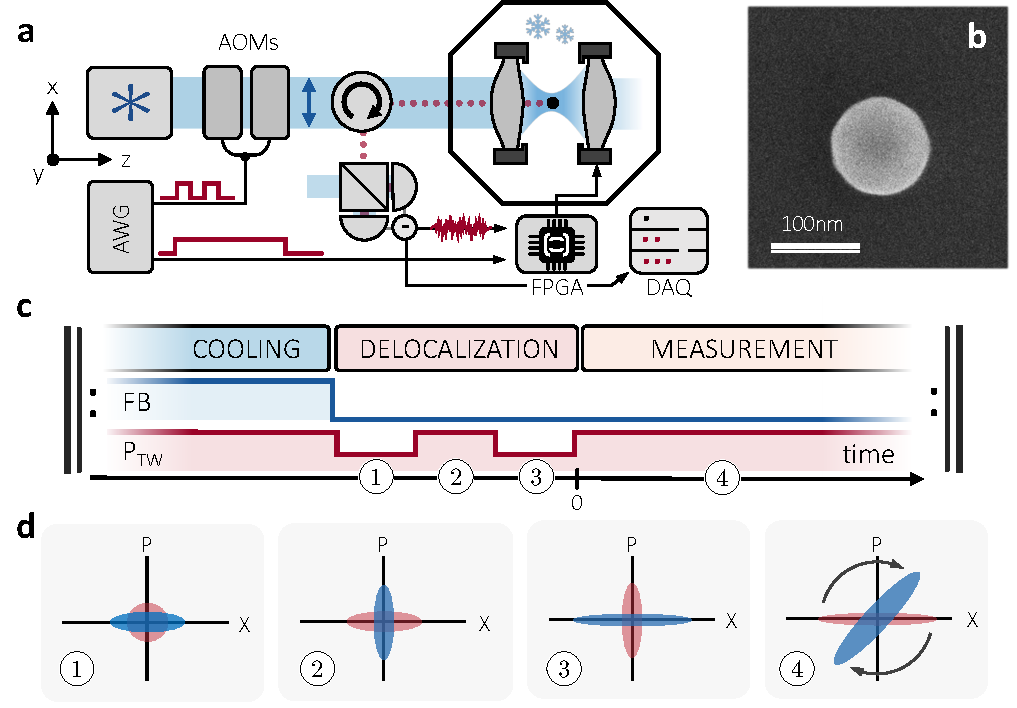
\includegraphics[width=86mm]{figures/figure1_05.pdf}
\caption{\textbf{Experimental setup and expansion protocol.} 
\textbf{a} Schematic overview of the optical and electronic setup. 
%
The power of the laser forming the tweezer is modulated by square waves.
%
The nanoparticle's motion is monitored by detecting the scattered photons and the corresponding signal is processed and acquired by digital electronics.
%
AOM, acousto-optic modulator; AWG, arbitrary waveform generator; DAQ, data acquisition card; FPGA, field-programmable gate array.
%
\textbf{b} Scanning electron microscope image of a nanoparticle.
%
\textbf{c} Steps for delocalizing the nanoparticle.
%
Feedback cooling is switched off during "delocalization" and "measurement".
%
The tweezer is modulated during "delocalization" only.
%
FB, feedback; $\mathrm{P_{TW}}$ tweezer power.
%
\textbf{d} Phase space distribution of the mechanical state during each step. 
%
The red (blue) ellipses represent the covariance matrix of the Gaussian state at the beginning (end) of the numbered phase of the experiment, in correspondence with \textbf{c}.}
\label{fig:experimental_setup}
\end{figure}
%
The essential elements of the experiment are illustrated in Fig.~\ref{fig:experimental_setup}a. 
%
We levitate a silica nanoparticle (nominal diameter \SI{100}{nm}, mass $m \approx \SI{1.2}{fg}$) inside a vacuum chamber by means of an optical tweezer propagating along the $z$ axis.
%
Figure~\ref{fig:experimental_setup}b shows a scanning electron microscope image of a typical particle. 
%
The optical tweezer is formed by focusing a linearly $x$-polarized laser beam (wavelength \SI{1550}{nm}, power $0.66\pm0.01~\mathrm{W}$) to a diffraction-limited volume with a single aspheric lens (numerical aperture 0.8).
%
For displacements of the nanoparticle much smaller than the laser wavelength, the center of mass motion along the three axes is decoupled from each other and harmonic with resonance frequencies $2\pi\times\{56.5,\,151.0,\,186.5\}\,$kHz, for the axes $\{z, x, y\}$ respectively.
%
In this work, we focus solely on the longitudinal motion along the $z$ axis and refer to its resonance frequency as $\Om$.
%
The lens holder is attached to the cold plate of a closed-cycle cryostat, which provides a temperature around the particle of \SI{7}{K} and a pressure below $10^{-9}$\,mbar.
%
Operating the system in ultra-high-vacuum makes the decoherence due to collisions with the background gas negligible (see Supplementary Material) \cite{tebbenjohanns_quantum_2021}.
%
\\
We monitor the displacement of the nanoparticle by detecting interferometrically the phase shift imprinted on backscattered photons.
%
This detection scheme is the most sensitive to measure the longitudinal motion \cite{tebbenjohanns_optimal_2019}.
%
From our position measurements, we estimate a total decoherence rate of $\Gamma_\mathrm{tot}=(23.7\pm 1.6)\times10^3\,\mathrm{phonons\,s^{-1}}$ and use this parameter to calibrate the data presented hereafter (see Supplementary Material).
%
The decoherence in our experiment is dominated by the random recoil due to photon scattering, also known as photon recoil (rate $\Gqba$) \cite{tebbenjohanns_quantum_2021,magrini_real-time_2021}.
\\
To cool the three motional modes of the nanoparticle and lower their energy, we generate a feedback signal from the acquired position measurement.
%
By driving three pairs of orthogonal electrodes and exploiting the electric charge carried by the nanoparticle, we can cool the transverse modes to a low occupancy thermal state, and the longitudinal one close to its ground state, with a residual average occupancy of $\overline{n} = 0.68\pm0.09$, measured via standard heterodyne thermometry techniques \cite{purdy_quantum_2017, tebbenjohanns_motional_2020}.
%
In the Supplementary, we also show additional datasets starting from different initial occupancies for the longitudinal motion.
\\
After cooling, the longitudinal motion of the nanoparticle is well localized. The uncertainty in its position is $\Delta z = \sqrt{(\overline{n}+1/2)} \zzpf \approx \SI{17}{pm}$ and the initial coherence length is $\xi_0\approx21\,\mathrm{pm}$, since the purity for a thermal state is $P=(2\bar{n}+1)^{-1}$.
%
In order to explore quantum mechanics at larger scales, we need to increase $\xi$, in other words to delocalize the nanoparticle motion while retaining its purity \cite{romero-isart_coherent_2017,weiss_large_2021}.
%
We do so by suddenly softening the trapping potential by reducing the focal intensity of the optical tweezer.
%
We perform this by means of an intensity modulator placed in the path of the optical tweezer before reaching the nanoparticle (see Supplementary Material).
%
The switching time of this modulator is around \SI{100}{ns}, a much faster timescale than the nanoparticle oscillation period of $\SI{18}{\mu s}$.

We design our experiment according to the following three-step protocol (shown in Fig.~\ref{fig:experimental_setup}c).
%
First, in the "cooling" step, we tune the laser intensity to the maximum value, corresponding to a mechanical resonance frequency $\Om$, and feedback cool the motion close to its ground state, with residual occupancy $\bar{n}$.
%
Once the steady state is attained, we move to the second step, the "delocalization". Here we switch the feedback off and modulate the trapping potential with a pulse sequence.
%
In the last step, "measurement", we reconstruct the delocalized state.
%
To that end, we toggle the laser intensity back to its maximum value and acquire the homodyne signal without applying any feedback.
%
We use the data acquired in this step to estimate the state generated at the end of the pulse sequence.
\\
To delocalize the nanoparticle, we employ a 2-pulse sequence.
%
These pulses (labels 1 and 3 in Fig.~\ref{fig:experimental_setup}c) lower the mechanical resonance frequency to $\Oe = \Om/r$, where $r$ denotes the frequency ratio. 
%
Their duration is $\pi/(2\Oe)$, i.e., a quarter of the lower mechanical period $2\pi/\Oe$.
%
During both pulses, the position uncertainty increases proportionally to the frequency ratio $r$, as sketched in Fig.~\ref{fig:experimental_setup}d \cite{janszky_strong_1992}.
%
Due to the lower impinging power, the decoherence rate due to photon recoil is reduced by a factor $r$.
%
We space these two pulses by a quarter of the original period, i.e., $\pi/(2\Om)$ (label 2 in Fig.~\ref{fig:experimental_setup}c).
%
During the time between the pulses, the nanoparticle oscillates at a rate $\Om$.
%
We introduce this spacing between the pulses to flip the sign of the average momentum that the nanoparticle has gained during the first pulse, e.g., due to stray static electric fields.
%
In this way, during the last pulse the nanoparticle continues to delocalize while containing the detrimental effect that drifting stray forces may have on the final state (see Supplementary Material).
%

We choose $r$=2.45 and repeat this experiment about 400 times.
%
In Fig.~\ref{fig:expanded_variance}a we show, for each repetition, the inferred nanoparticle's motion in units of zero point motion.
%
The initial time $t=0\,\mathrm{\mu s}$ corresponds to the beginning of the "measurement" step.
%
\begin{figure}[tbp]
\begin{center}
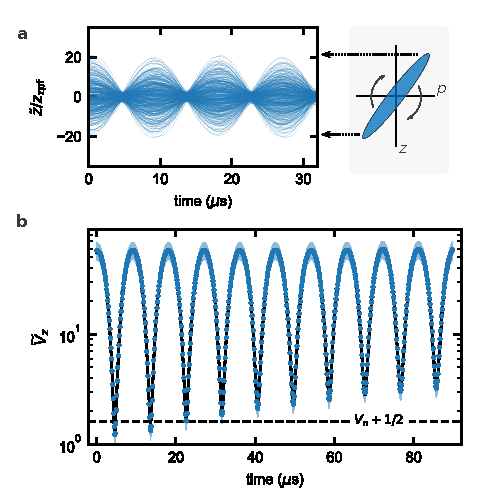
\includegraphics[width=86mm]{figures/figure2_G39_03.pdf}
\caption{\textbf{State evolution after recapture.}
\textbf{a} Ensemble of about 400 filtered trajectories.
%
The zero of the time axis corresponds to the beginning of the "measurement" step.
%
The phase space diagram on the right illustrates the dynamics of the generated state.
%
\textbf{b} Ensemble variance of the position as a function of time (circles), and fit (black line). 
%
The blue shaded area represents the 95\% confidence on the data.
%
The horizontal dashed line represents the sum between the variance of the zero point motion ($1/2$) and our measurement uncertainty ($V_n$).}
\label{fig:expanded_variance}
\end{center}
\end{figure}
%
To extract the trajectory, we filter in two steps the raw homodyne signal acquired during the "measurement" step.
%
First, we apply backward in time a pair of second-order high-pass filters to reject noise in the low frequency part of the spectrum (cutoff $3\,\mathrm{kHz}$ and $9\,\mathrm{kHz}$).
%
Then, we apply a retrodiction filter based on a stochastic master equation to optimally infer the motion down to the beginning of the "measurement" step \cite{rossi_observing_2019, lammers_quantum_2024}.
%
Each of the trajectories shown in Fig.~\ref{fig:expanded_variance}a is the output of such a retrodiction filter.
\\
From the data, we can qualitatively deduce that the position uncertainty (the spread of trajectories) oscillates at $2\Om$.
%
This is consistent with an asymmetric position-momentum (phase space) distribution.
%
This distribution rotates in the phase space at a rate $\Om$.
%
Consequently, its position marginal oscillates at twice that rate (cf. inset of Fig.~\ref{fig:expanded_variance}a).
%
We calculate at each time step the position ensemble variance, $\widetilde{V}_z$, over the 400 realizations shown in Fig.~\ref{fig:expanded_variance}b.
%
Hereafter, we refer to estimated quantities (either from experiment or theory) with a tilde.
%
In addition to the oscillations at $2\Om$, we observe that the minimum variance increases with time.
%
This increase is due to the photon recoil.
%
To quantify the maximum delocalization, we fit the data up to $360\,\mathrm{\mu s}$ to the following model (see Supplementary Material for its derivation)
%
\begin{eqnarray}
\label{eq: variance in time}
\widetilde{V}_z(t) &= \widetilde{V}_z(0)\cos\left(\Om t\right)^2+\widetilde{V}_p(0)\sin\left(\Om t\right)^2 + \\
&+\widetilde{C}_{zp}(0)\sin\left(2\Om t\right) + \Gqba \left(t-\frac{\sin\left(2\Om t\right)}{2\Om}\right), \nonumber
\end{eqnarray}
where $\widetilde{V}_z(0), \widetilde{V}_p(0)$ and $\widetilde{C}_{zp}(0)$ are, respectively, the estimated position and momentum variances and the symmetrized covariance at time $t=0\,\mathrm{\mu s}$.
%
In Eq.~\eqref{eq: variance in time}, the position and momentum are normalized to their corresponding zero point motion $\zzpf$ and $\pzpf=\hbar\zzpf^{-1}$, respectively.
%
We notice that both variance estimates are biased by the same estimation noise $V_n$, i.e., $\widetilde{V}_z(0)=V_z(0)+V_{n}$ and $\widetilde{V}_p(0)=V_p(0)+V_{n}$.
%
This bias originates from imprecision noise in the measurement that the filter cannot reject \cite{wieczorek_optimal_2015, rossi_observing_2019, lammers_quantum_2024}.
%
From our parameters, we find that $V_n=(1.1\pm0.1)$.
For reference a perfectly efficient measurement would yield $V_n=0.5$.
%
This is because our apparatus operates in the weak measurement regime ($\Gqba/\Om\approx0.07\ll1$), and is effectively equivalent to a simultaneous position and momentum measurement \cite{doherty_quantum_2012}.
%
The finite estimation noise ensures that the Heisenberg principle is fulfilled.
%
From the fits, we obtain the covariance matrix of the delocalized mechanical state.
%
In principle, this covariance matrix should be diagonal, with the position variance as the largest value.
%
In practice, small inaccuracies in the pulses' duration might generate a mechanical state with finite correlations between position and momentum, with the largest delocalization in a rotated quadrature ($\delta\tilde{\theta}\approx0.02 \pi$).
%
We find this delocalization by extracting the maximum eigenvalues of the estimated covariance matrix. 
%
For the sake of simplicity, we keep referring to the maximum and minimum eigenvalues as the position and momentum variance, respectively.
%
For this experiment, we find $\widetilde{V}_z=56\pm6$. This corresponds to a position uncertainty of $\Delta z= (120\pm6)\,\mathrm{pm}$, seven times the initial uncertainty of $17\,\mathrm{pm}$.
\\
We repeat the measurement outlined above for different frequency ratios $r$ and show the results in Fig.~\ref{fig:expansion_vs_r}.
%
\begin{figure}[tbp]
\begin{center}
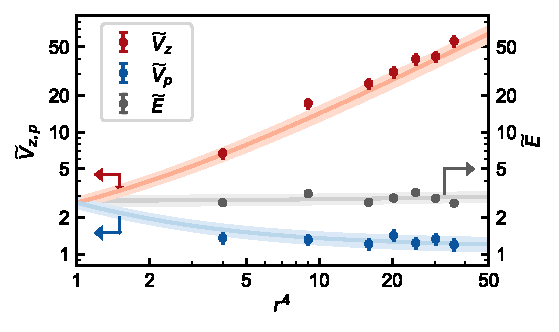
\includegraphics[width=86mm]{figures/figure3_G39_04.pdf}
\caption{\textbf{Estimated variance and energy after delocalization and recompression.}
The red and blue circles are, respectively, the estimated position and momentum variances after the delocalization, and refer to the left vertical axis. 
%
The datapoints for $\widetilde{V}_z$ and $\widetilde{V}_p$ at the highest $r$ are obtained from the data shown in Fig.~\ref{fig:expanded_variance}.
%
The gray circles represent the total energy of the particle after recompression and refer to the right vertical axis. 
%
The error bars on the experimental data represent the 95\% confidence interval deduced from the fit parameters. 
%
The solid coloured lines are theoretical predictions and the shaded areas reflect the 95\% confidence interval of the model parameters.}
\label{fig:expansion_vs_r}
\end{center}
\end{figure}
%
The red and blue circles represent, respectively, the maximum and minimum eigenvalues of the estimated covariance matrix.
%
We observe that the position variance scales with the fourth power of the frequency ratio, $r^4$, whereas the estimated momentum variance approaches the estimation noise $V_n$.
%
To account for these data, we model our experiment by standard optomechanical theory in free space \cite{militaru_ponderomotive_2022}.
%
From this model, we predict
%
\begin{subequations}
\label{eq: state prediction}
\begin{align}
\widetilde{V}_{z,\mathrm{th}} &= V_n + r^4 V_0 + \frac{\Gqba}{\Om}\frac{\pi}{2}\left(r+r^2+r^3\right),\label{eq:vzest_th}\\
\widetilde{V}_{p,\mathrm{th}} &= V_n + r^{-4} V_0 + \frac{\Gqba}{\Om}\frac{\pi}{2}\left(r^{-1}+r^{-2}+r^{-3}\right),\label{eq:vpst_th}
\end{align}
\end{subequations}
%
where $V_0=\bar{n}+1/2$ and $\bar{n}$ is the initial phonon occupancy (due to feedback cooling).
%
In particular, note that we assume photon recoil as the only significant decoherence throughout the experiment, i.e., $\Gtot\approx\Gqba$.
%
The solid lines in Fig.~\ref{fig:expansion_vs_r} are predictions from the model without fitting parameters.
%
The shaded area reflects the uncertainty in the independently measured parameters used to evaluate Eqs.~\eqref{eq: state prediction}.
%
The good agreement between experiment and theory supports the assumption that decoherence effects besides photon recoil are negligible in our experiment.
\\
These data show an increase in the position uncertainty. 
%
To verify that the prepared state has not lost coherence,  we perform the following experiment: we delocalize and immediately compress the nanoparticle state back \cite{weiss_large_2021}.
%
For this experiment, we change the duration of the pulse sequence: we double the length of the two pulses, i.e., $\pi/\Oe$, and shorten their spacing to the minimum possible amount in practice, i.e., $\sim200\,\mathrm{ns}$ limited by the AOM switching time.
%
In this way, we approach a single pulse of duration $2\pi/\Oe$.
%
Since this duration is the period of the dynamics during the pulse, the final state equals the initial one.
%
We leave the measurement and estimation steps unchanged.
%
In Fig.~\ref{fig:expansion_vs_r} we show the estimated energy of the final state as gray circles.
%
We derive the energy from the position and momentum variance as $\widetilde{E}=(\widetilde{V}_z+\widetilde{V}_p)/2$.
%
In absence of decoherence, the total mechanical energy at the end is unchanged and the purity unaffected.
%
In practice, the residual decoherence due to photon recoil slightly increases the nanoparticle energy, after the protocol.
%
From our model, we predict for the estimated energy after the protocol $\widetilde{E}_\mathrm{th}=V_n+V_0+\Gqba(\Om \pi)^{-1} \left(r+r^{-1}\right)$.
%
We compute this prediction and show it as a solid line in Fig.~\ref{fig:expansion_vs_r}, with the shaded area reflecting the uncertainty in the parameters used to evaluate it.
%
The good agreement between prediction and experiment supports, once more, our assumption that photon recoil is the dominant process during delocalization.


To further support our claim of having prepared a state delocalized beyond the zero-point motion, we infer from the previous dataset the coherence length.
The state we generate presents, at time $0\,\mathrm{\mu s}$, negligible correlations between position and momentum.
Thus, the coherence length can be further simplified and expressed as $\xi=\zzpf\sqrt{2/V_p}$.
To infer the  momentum variance, we subtract from the estimated one $\widetilde{V}_p$ (from Fig.~\ref{fig:expansion_vs_r})  the estimation noise $V_n$.
In order to get meaningful errorbars for the variance, i.e., corresponding to a physically realizable state, we use a positive semidefinite optimization to perform the subtraction and a Montecarlo method to obtain a 95\% confidence interval \cite{kotler_direct_2021} (see also Supplemental Material).
%
We show in 
Fig.~\ref{fig:coherence length} the inferred coherence length for the different ratios $r$.
\begin{figure}[tbp]
\begin{center}
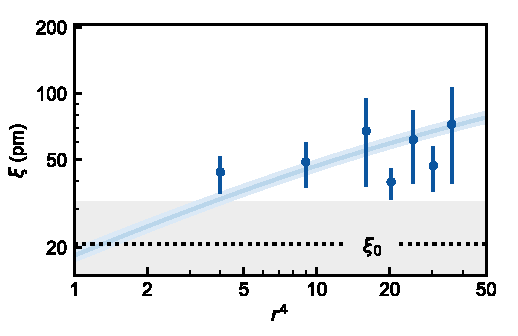
\includegraphics[width=86mm]{figures/figure4_G39_05.pdf}
\caption{\textbf{Inferred coherence length.}
The circles are inferred coherence lengths and the error bars represent the 95\% confidence interval of the estimates.
The blue solid line is the prediction from our model, and the shaded area reflects the 95\% confidence interval in the model parameters.
The gray area bounds the region of coherence lengths obtainable with ground-state cooling.
The dashed line marks the initial coherence length.}
\label{fig:coherence length}
\end{center}
\end{figure}
%
We observe that the inferred coherence length is always larger than its initial value.
%
In particular, we notice that for large $r$ it exceeds the coherence length of the ground state.
%
For the highest $r$, we have $\xi=(73\pm34)\,\mathrm{pm}$, more than a threefold increase compared to the initial state ($\xi_0\approx~21\,\mathrm{pm}$) and doubling the zero-temperature state coherence length ($\xi_{|0\rangle}\approx~32\,\mathrm{pm}$).
%
Our system exceeds the ground state coherence length due to the squeezed momentum fluctuations below the zero point value \cite{wollman_quantum_2015, pirkkalainen_squeezing_2015, youssefi_squeezed_2023}. Indeed, we find that momentum variance is squeezed by $-7.2^{+2.9}_{-11.5}\,\mathrm{dB}$ below its zero-point value.
% $$ $\Delta p/p_\mathrm{zpf}=0.44\pm0.20$, which corresponds to a squeezing of the momentum standard deviation by more than a factor of 2.

Our results show a coherent delocalization of the position of a levitated nanosphere to $73\,\mathrm{pm}$.
%
This stems from the increased position uncertainty and a preserved state purity.
%
The observed excess noise is consistent with decoherence caused by quantum backaction due to photon scattering during the delocalization protocol.
%
To go to even larger coherence length, the next step to reduce this decoherence by implementing "dark" traps for the expansion protocol \cite{pino_-chip_2018,roda-llordes_macroscopic_2023}, such as RF traps \cite{conangla_extending_2020, bykov_hybrid_2022}. 
%
The use of such a hybrid trap has recently been demonstrated in the context of  classical state expansion \cite{bonvin_state_2023}.
%
To the best of our knowledge, there are no fundamental limitations to the application of the quantum control techniques developed in this work with the hybrid trap of Ref.~\cite{bonvin_state_2023}. 
%
The squeezing that underlies the enhanced coherence length  provides an advantage in force sensing \cite{burd_quantum_2019}, e.g., for the detection of small electric forces. 
%
Moreover, the methods presented here are important for elucidating open questions at the interface of quantum physics and gravity, such as the gravitational coupling of two delocalized quantum masses \cite{dewitt_role_2011, marletto_gravitationally_2017, bose_spin_2017, belenchia_quantum_2018}.

\textbf{Acknowledgments} We thank the Q-Xtreme synergy group and our colleagues at the ETH photonics laboratory for fruitful discussions. This research has been supported by the European Research Council (ERC) under the grant agreement No. [951234] (Q-Xtreme ERC-2020-SyG), the Swiss SERI Quantum Initiative (grant no. UeM019-2) and the Swiss National Science Foundation (grant no. 51NF40-160591). N.C.Z. thanks for support through an ETH Fellowship (grant no. 222-1 FEL-30). A.R.-C. acknowledges funding from the European Union’s Horizon 2020 research and innovation programme under the Marie Skłodowska-Curie grant agreement No. [101103589] (DecoXtreme, HORIZON-MSCA-2022-PF-01-01).

\textbf{Author Contributions} 
M.R. led the project.
% M.R., O.R.-I. and L.N. conceived the idea.
M.R., A.M. and N.C.Z. designed the experiment, built the setup, acquired and analyzed the data in equal contribution. Together with M.F. and L.N., they discussed the results. A.R.-C. and O.R.-I. provided support with the theoretical modeling. All authors contributed to writing the manuscript. O.R.-I. and L.N. gave the research direction and vision. L.N. supervised the project.

\bibliography{main.bib}
\bibliographystyle{naturemag}

\end{document}